\documentclass[kul]{kulakbeamer}
\usepackage[english]{babel}
\usepackage[utf8]{inputenc}
\usepackage[T1]{fontenc}


\title[Bolts vs. Shields]{Restraining Bolts vs Shielding}
\subtitle{Safe Reinforcement Learning}
\author[Robbe \& Elias]{Robbe Louage \& Elias Storme}
\date{11th of March 2020}
\institute[Dept. CW]{Dept. Computerwetenschappen}

%% Overview at begin of each section; delete if unwanted.

\AtBeginSection[]{
	\begin{outlineframe}[Outline]
	%\frametitle{Outline} %Change to "Outline" for English presentation
	{
		\hypersetup{hidelinks} %disable link colors
		\hfill	{\large\parbox{.95\textwidth}{\tableofcontents[currentsection,hideothersubsections]}}
	}
\end{outlineframe}}
\addtobeamertemplate{footline}{\hfill\usebeamertemplate***{navigation symbols}%
    \hspace*{0.1cm}\par\vskip 2pt}{}

\begin{document}

\begin{titleframe}
\titlepage
\end{titleframe}

 % % % Here you go  % % % 
\begin{outlineframe}[Outline]
	{
		\hypersetup{hidelinks} %disable link colors
		\hfill	{\large\parbox{.95\textwidth}{\tableofcontents[hidesubsections]}}
	}
\end{outlineframe}

\section{Introduction}
\begin{frame}
\frametitle{Motivation}
\begin{itemize}
    \item Good convergence and optimality not always main concern
    \item Safe operation may be more important
    \item Needed:
    \begin{itemize}
        \item Formal way to specify what is safe
        \item Enforcement mechanism for that specification
    \end{itemize}
\end{itemize}
\end{frame}
\section{Preliminaries}
\subsection{Safety Specification}
\begin{frame}
\frametitle{$LTL_F/LDL_F$}
\begin{itemize}
    \item finite linear-time temporal logic (Pnueli 1977)
    \item encode formulae about the future of paths
    \item built from propositional variables, logical operators ($\lnot,\lor, ...$) and temporal model operators \textbf{X,U G, F, R, W, M}
    \item \textbf{X}=Next, \textbf{U}=until, \textbf{G}=Globally, ...
    
\end{itemize}
\end{frame}

\begin{frame}
\frametitle{Some examples}
\begin{itemize}
    \item Safety: “something bad will not happen” \\
    \textbf{G}$(reactor\_temp> 1000)$ \\
    \textbf{X} valve\_open $\implies$ water\_level > 10 
    \item Liveness: “something good will happen” \\
    \textbf{G}(start $\implies$ \textbf{F} terminate)
\end{itemize}
\end{frame}


\begin{frame}
\frametitle{Safety Automaton}
 \begin{itemize}
     \item How to implement $LTL_f$ formulas?
     \item In reinforcement learning an agent must learn a behaviour through trial and error via interaction with a
     environment modelled by a MDP $M=(S,s_i,A,P,R)$.
     \item A specification $\rho$ defines a set of allowed paths (traces). 
     \item a specification is said to be safe $iff$ every path that is not allowed has a prefix such that all other paths with that prefix are also not allowed.
     \item for specification in LTL it is know how to compute a safety automaton that represents it (Kupferman and Vardi 2001) 
     \item $\rho^{s} = (Q,q_0,\Sigma, \delta, F)$
     \item F is a subset of Q, all states in F are safe.
 \end{itemize}
\end{frame}
\subsection{Environment}

\section{Approaches}
\subsection{Restraining Bolts}
\begin{frame}
\frametitle{Restraining Bolts}
   \begin{figure}
    \centering
    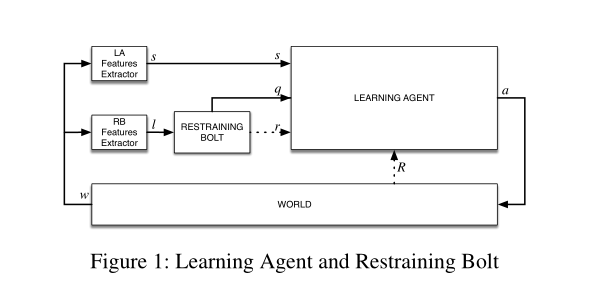
\includegraphics[scale=0.6]{bolts.png}
    \end{figure}
    \begin{itemize}
        \item  a simulator of the dynamic system
        \item a re-strainingbolt (RB) process
        \item a reinforcement learning (RL) agent
        \item modular
         \item satisfy the RB specifications when enough training is allowed
    \end{itemize}

\end{frame}

\subsection{Shielding}
\begin{frame}{Shielding}
    \begin{itemize}
        \item Shield = (finite state) safety automaton
        \item Observes the world
        \item Enforces safety specification on learner
    \end{itemize}
\end{frame}
\begin{frame}{Shielding: schematically}
    \begin{figure}
        \centering
        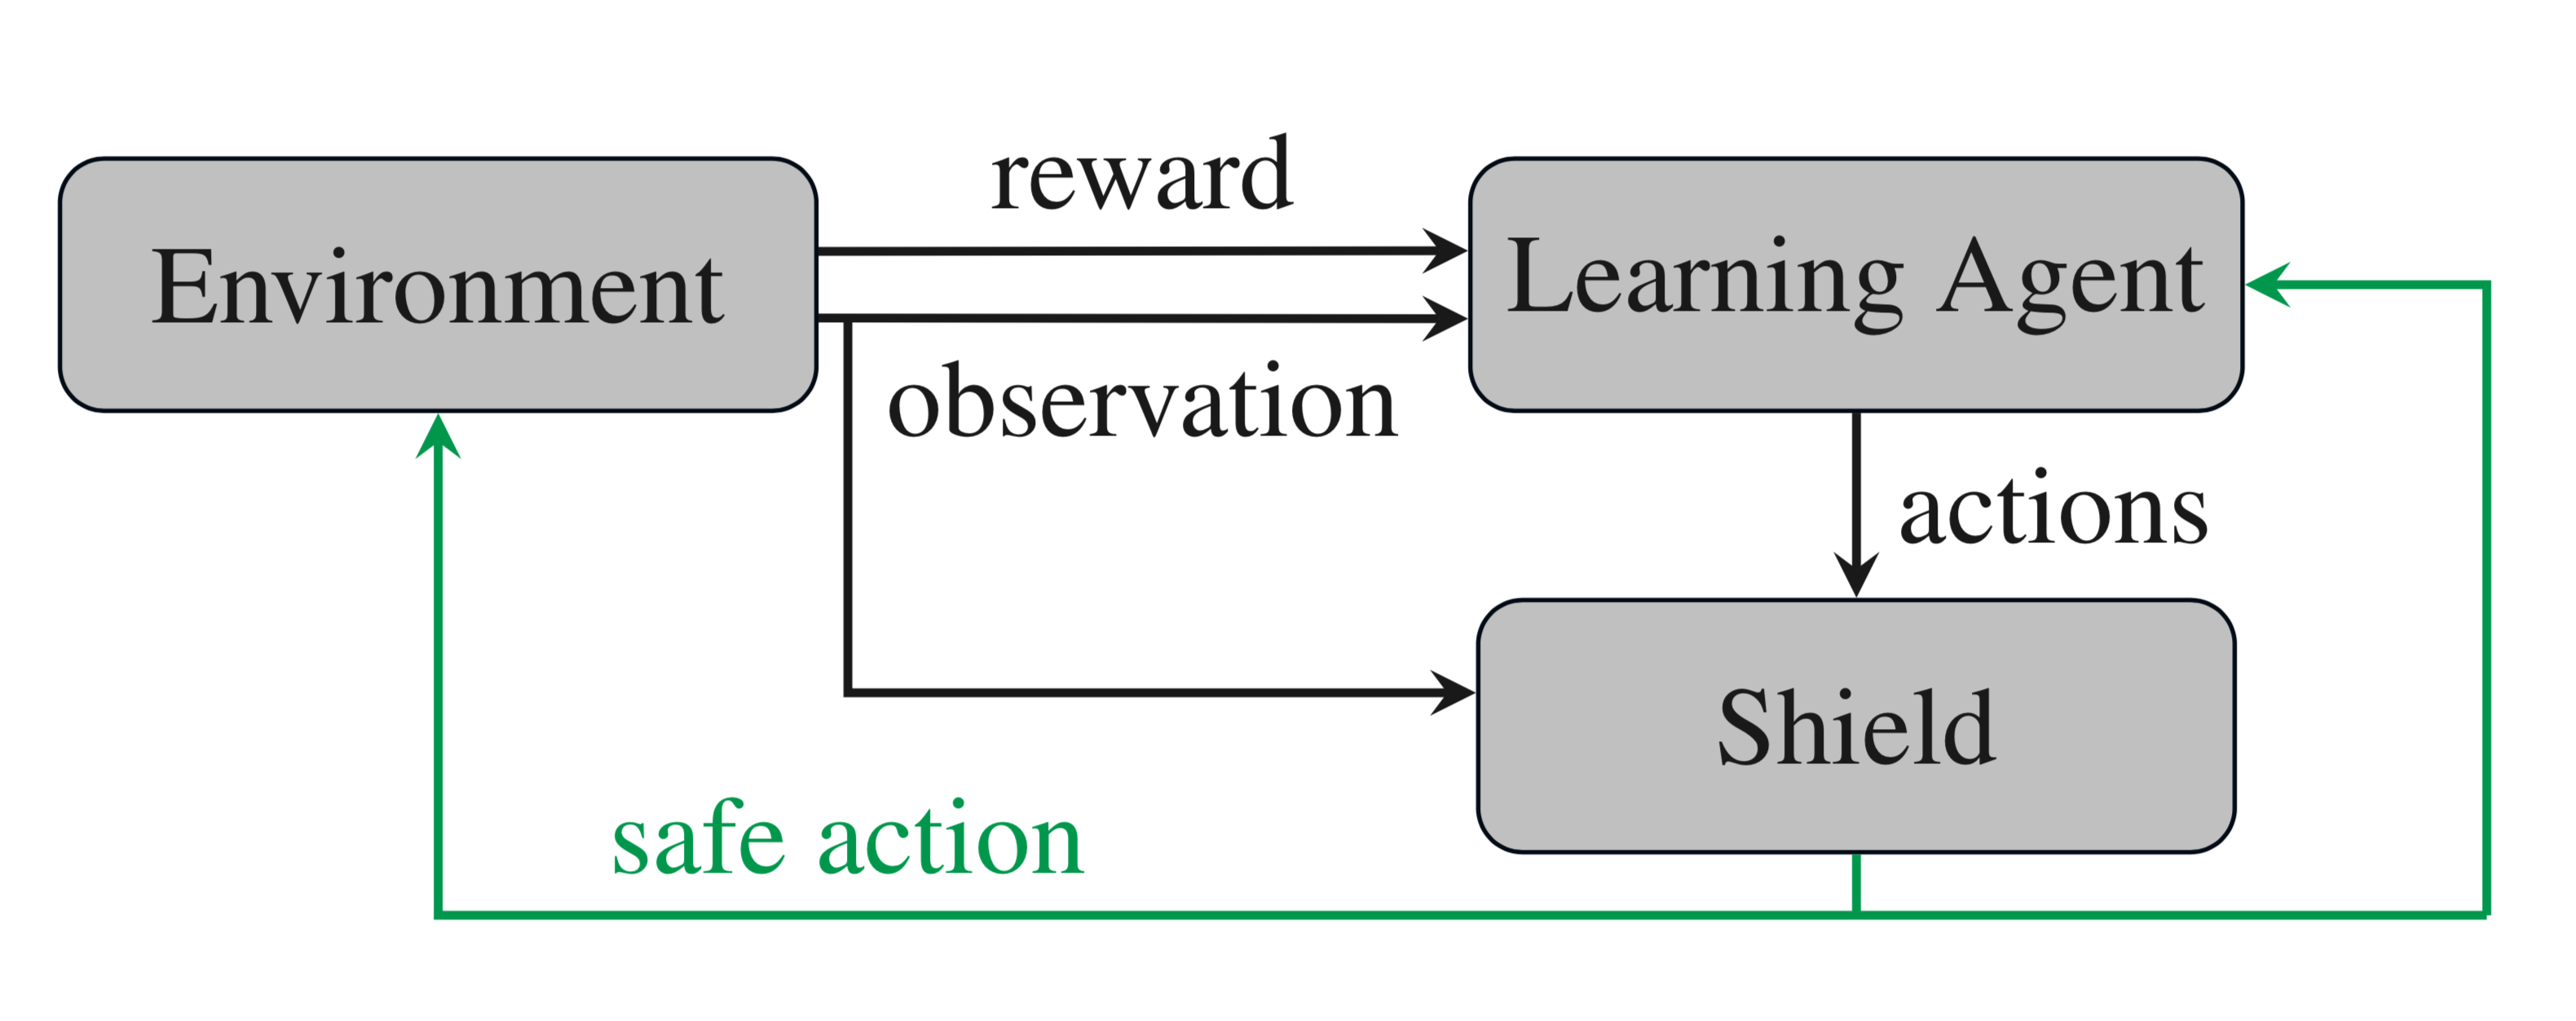
\includegraphics[width=\textwidth]{Shielding.png}
    \end{figure}
\end{frame}
\begin{frame}{Shielding}
    \begin{itemize}
        \item Similar approach as restraining bolt
        \item Crucial difference: agent submits action to shield
        \item Shield can then:
        \begin{itemize}
            \item If safe: pass action to environment
            \item If unsafe: replace with safe action
        \end{itemize}
        \item Reward strategy: 2 approaches
        \begin{itemize}
            \item Assign punishment
            \item Assign reward of substituted action
        \end{itemize}
    \end{itemize}
\end{frame}
\subsection{Similarities}
\begin{frame}{Similarities}
    \begin{itemize}
        \item Specification language
        \item Result: use automata to enforce safety
        \item Resulting learning environment: Non-Markovian Reward Decision Process
        \item Learner independence
    \end{itemize}
\end{frame}
\subsection{Differences}

\begin{frame}
\frametitle{Restraining bolts: advantages}
\begin{itemize}
    \item Simplicity in enforcement
    \item No need to make automaton anticipate future
    \item Environment observation may be less complex
\end{itemize}
\end{frame}
\begin{frame}{Restraining bolts: advantages}
   \begin{figure}
    \centering
    \def\svgwidth{.8\columnwidth}
    \input{Breakout.pdf_tex}\footnotemark
\end{figure}
\footnotetext{Image source: Wikimedia}
\end{frame}
\begin{frame}
\frametitle{Shielding: advantages}
    \begin{itemize}
        \item Learner cannot break safety specification
        \item Restraining bolt has no 100\% guarantee no unsafe behavior will occur
    \end{itemize}
\end{frame}

\section{Creative part}
\subsection{Sapientino}
\begin{frame}{Sapientino}
    Children's board game
    \begin{figure}
        \centering
        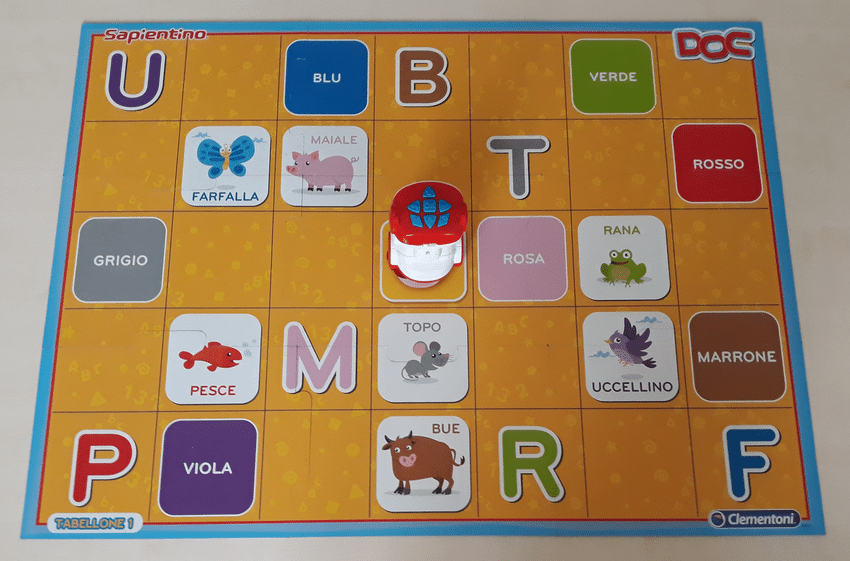
\includegraphics[width=.8\textwidth]{sapientino.png}
    \end{figure}
\end{frame}
\begin{frame}{Sapientino}
    \begin{itemize}
        \item Safety specification:
        \begin{itemize}
            \item Bip colors in triplets, in specific order
            \item Red, green, blue, pink, brown, gray, purple 
        \end{itemize}{}
        \item Crucial point making game suitable: safe trace broken by one action
    \end{itemize}{}
\end{frame}{}
\subsection{Results}
\begin{frame}{Convergence}
    \begin{figure}
        \centering
        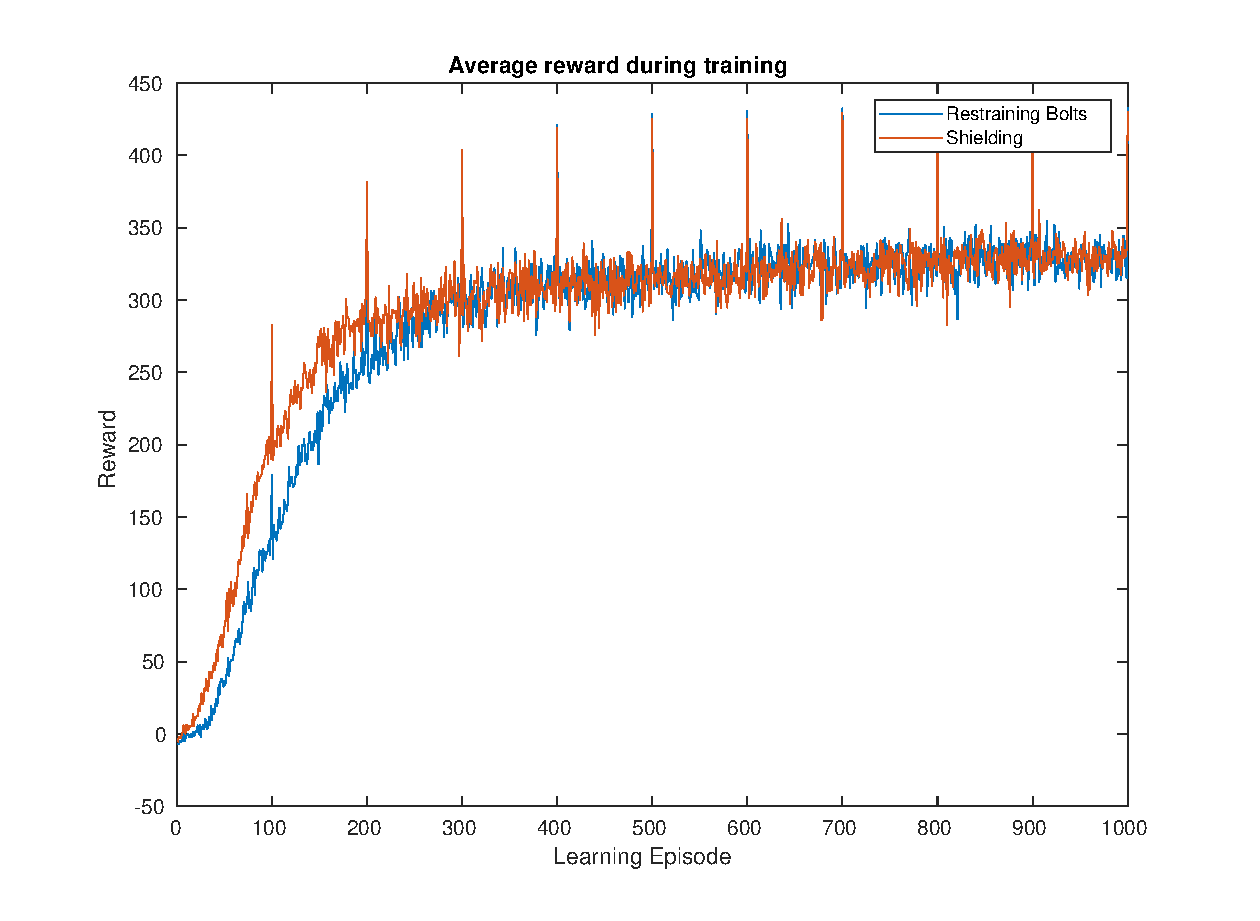
\includegraphics[width=.87\textwidth]{learning_reward.eps}
    \end{figure}{}
\end{frame}{}
\begin{frame}{Policy reward}
    \begin{figure}
        \centering
        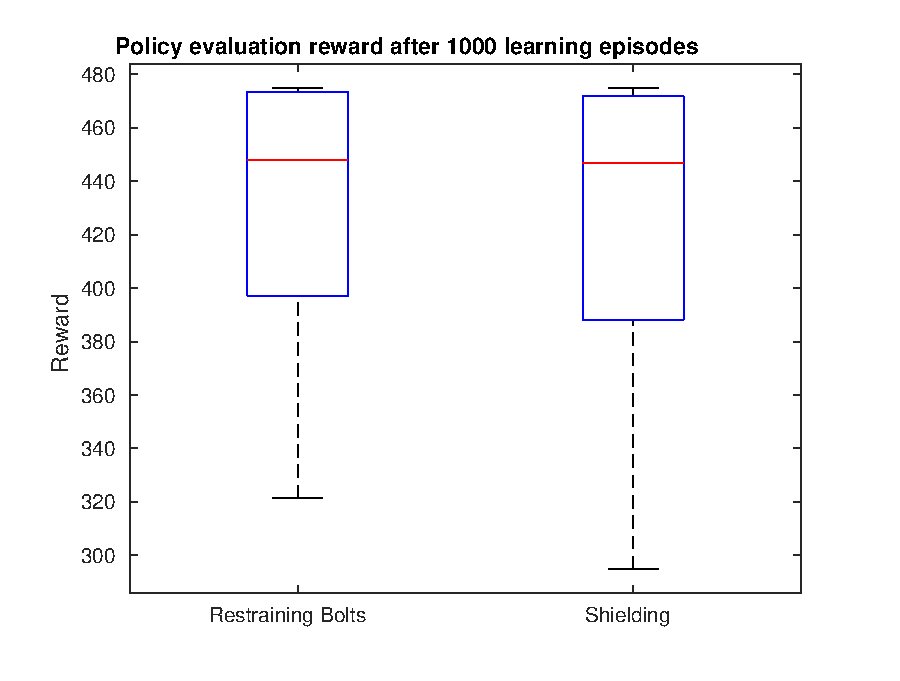
\includegraphics[width=.84\textwidth]{policy_reward.eps}
    \end{figure}{}
\end{frame}{}
\begin{frame}{Policy number of actions}
    \begin{figure}
        \centering
        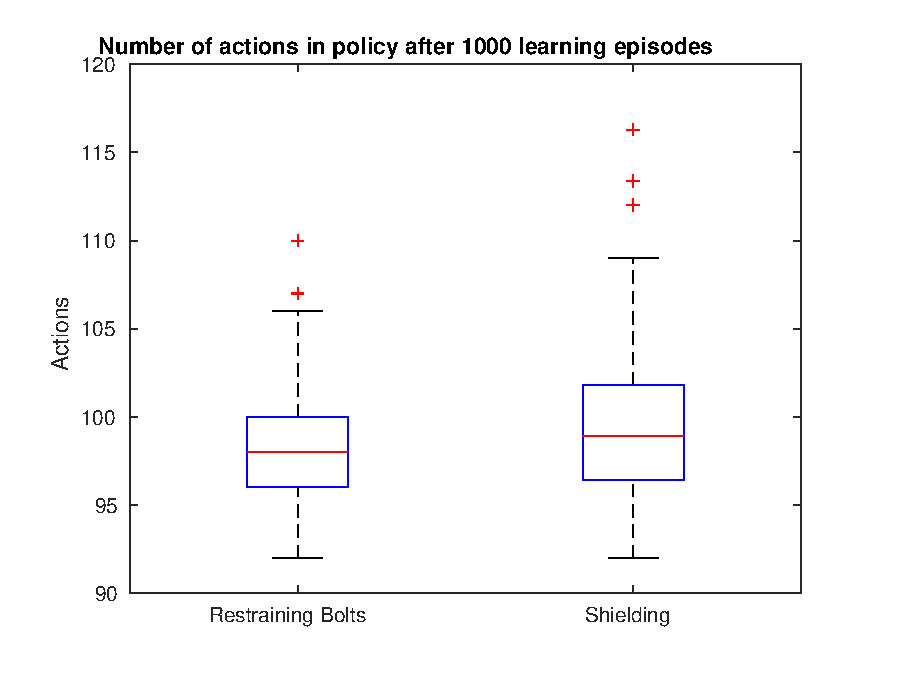
\includegraphics[width=.84\textwidth]{policy_actions.eps}
    \end{figure}{}
\end{frame}{}
\begin{frame}{Takeaway}
    \begin{itemize}
        \item Resulting policy may contain more useless actions using shielding
    \end{itemize}
\end{frame}
\section{Conclusion}
\begin{frame}
\frametitle{Conclusions}
\begin{itemize}
    \item RB generally achieve higher rewards and a lower number of total actions per episode when training and executing.
    \item RB does not guarantee hard prevention of actions, shield do guarantee this.
    \item RB specifications are generally easier to write because the future does not have to be computed. (In some cases this can be very hard or even impossible)
    %\item Predictions are very hard to make, especially about the future!
\end{itemize}
\end{frame}

\end{document}